\section*{WRITING TASK 1}
You should spend about 20 minutes on this task.

\begin{quote}\large The bar chart compares the percentages of commuters using four main forms of transport in Bellford in 2005 and 2025.
\end{quote}
Describe the main features of the information, select relevant details, and make comparisons where appropriate.

\begin{center}
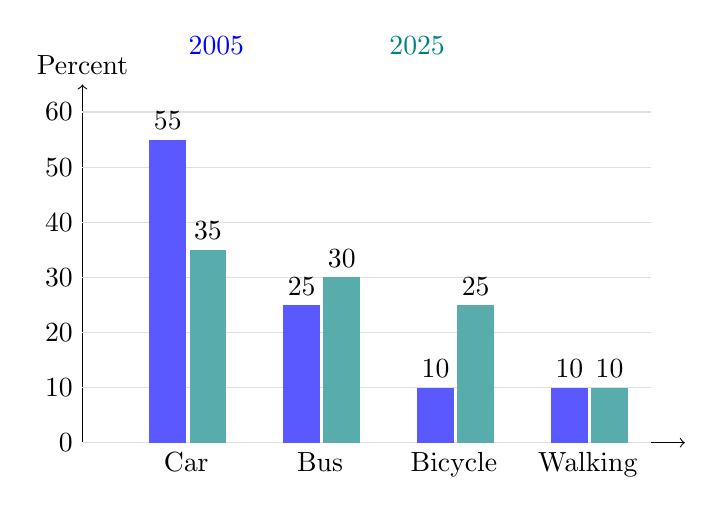
\begin{tikzpicture}[x=0.85cm,y=0.07cm]
\draw[->] (0,0)--(9,0);\draw[->] (0,0)--(0,65) node[above]{Percent};
\foreach \v in {0,10,20,30,40,50,60}{\draw[gray!25] (0,\v)--(8.5,\v);\node[left] at (0,\v){\v};}
\foreach \x/\a/\b/\name in {1/55/35/Car,3/25/30/Bus,5/10/25/Bicycle,7/10/10/Walking}{
\fill[blue!65] (\x,0) rectangle +(0.55,\a);\fill[teal!65] (\x+0.6,0) rectangle +(0.55,\b);
\node[above] at (\x+0.275,\a){\a};\node[above] at (\x+0.875,\b){\b};\node[below] at (\x+0.55,0){\name};}
\node[blue] at (2,72){2005};\node[teal] at (5,72){2025};
\end{tikzpicture}
\end{center}
Write at least 150 words.
\par\bigskip
{\footnotesize\color{gray} Original practice material; fictional settings and data. Not an official IELTS examination paper.}
